\section{Introduction}
\label{sec:accurate_pdet_intro}

As described in \Cref{cha:first_paper} future missions are expected to use
orbital information collected from radial velocity (RV) fits to create their
initial observation schedule. Directly imaging an Earth-like planet is very
dependent on the planet's position along its orbit because its orbital phase
determines the amount of light reflecting off the planet and the fact that at
smaller angular separation's $\alpha$ a telescope will collect less of the planet's
light. In \Cref{cha:first_paper} a method of creating orbits consistent
with the underlying radial velocity data was detailed and the probability
of detection was calculated as
\begin{equation}
    P_{\textrm{det}}(t) = \frac{\textrm{Number of orbits detectable at time $t$}}{\textrm{Number of
    constructed orbits}}
.\end{equation}
This equation is an accurate description of the probability of detection
$P_\textrm{det}$, however the "Number of orbits detectable at time $t$" factor
was hiding a lot of complexity. The constraints used to establish whether an orbit
was detectable were
\begin{align}
    \text{IWA} < \alpha < \text{OWA}\\
    \Delta\mathrm{mag} < \Delta\mathrm{mag}_0
\end{align}
where the $\Delta\textrm{mag}_0$ value is the flat instrument noise floor,
$\Delta\textrm{mag}$ is the planet-star difference in brightness magnitude, IWA
is the instrument's inner working angle, and OWA is the instrument's outer
working angle.

\Cref{cha:coupling} we described that using a flat value of
$\Delta\textrm{mag}_0$ will overestimate completeness and described how we can
calculate $\Delta\textrm{mag}_0$ as a function of various astrophysical inputs,
primarily the integration time $t_\textrm{int}$ and $\alpha$ when using an
optical system where the planet and background signals are coupled. Calculating
completeness as a function of more than the noise floor is a very
computationally demanding task, in an already computationally demanding process
of yield modeling, and many yield modeling tools and scheduling algorithms have
been built on the assumption of a flat limiting $\Delta\textrm{mag}_0$
\citep{savranskyAnalyzingDesignsPlanetFinding2010,starkMaximizingExoEarthCandidate2014,
keithlyOptimalScheduling2020, garrettAnalyticalFormulation2016,
keithlyIntegrationTime2021, morganFasterExoEarth2021}.

Completeness has traditionally been used by yield modeling tools to establish
promising targets for a blind-search mission simulated as Monte Carlo
Mission Simulations \citep{savranskyEXOSIMSExoplanetOpenSource2017}
and to estimate yield by summing mission completeness
\citep{Brown2005d}. Both
methods rely on rapid computation, sacrificing accuracy in the calculation of
completeness to allow for a better understanding of the mission design trade
space.

The work of this chapter is to generate the most accurate probability of
directly imaging a planet for an individual observation. However, it is useful
to analyze the impact of different astrophysical inputs on the completeness
metric as it can help drive our intuition for $P_\textrm{det}$.

In \Cref{sec:impact_on_completeness} we  first demonstrate the impact of
assuming a flat $\Delta\textrm{mag}_0$ value for calculations of completeness
and then expand $\Delta\textrm{mag}_0$ to account for zodiacal and exozodiacal light. Then in
\Cref{section:impact_on_pdet} we will apply the improved $\Delta\textrm{mag}_0$ values to the probability of
detection metric $P_\textrm{det}$ that was described in \Cref{cha:first_paper},
ultimately expanding $P_\textrm{det}$ to account for variations in $t_\textrm{int}$, $\alpha$,
local zodiacal light, and exozodiacal light.

% For example, the paper \citet{keithlyIntegrationTime2021} created a method
% of calculating complenetess
% The paper \citet{starkExoEarthYieldLandscape2019} calculates the contrast
% limit as a function of $\alpha$ but then assumes a flat noise floor due
% to an improvement in signal based on post-processing

\section{Impact of Separation and Zodiacal Light on Completeness}
\label{sec:impact_on_completeness}

Completeness represents the probability of detecting a set of planets from a
given population for a given telescope design. As NASA's currently stated goal
is to detect Earth-like planets \citep{nasaNASAStrategic2022} that will be the planet population of interest
here. The parameters for the telescope shown in the rest of the chapter are
taken from \citet{morganExplorationExpectedNumber2022a} which aimed to simulate
the yield of a 6 m telescope similar to the proposed Habitable Worlds
Observatory.

Yield estimates based on summed completeness are useful because they are much
faster than running full mission simulations. Typically they have been used to
study the effect of many different astrophysical inputs on mission yield
\citep{starkMaximizingExoEarthCandidate2014, Stark2016,
starkExoEarthYieldLandscape2019}. The standard way to calculate summed
completeness for a mission is to calculate the completeness per integration
time and then assign observation time to the most beneficial stars
\citep{hunyadiSingleVisitCompleteness2005,
starkMaximizingExoEarthCandidate2014}. After allocating observation time to
each target star it is a simple matter of summing the completeness for all
targets at their allocated observation time.

% In \citet{starkExoEarthYieldLandscape2019} the instrument's contrast limit was
% treated as a function of separation by calculating the core throughput at a
% planet's separation and using that to determine the limiting contrast, however
% it is difficult to discern what exactly the completeness constraints were because
% there is an additional note saying that the post-processing noise floor is held to a constant
% value and the code itself is not open source. Either way, 

With the coupling described in \Cref{cha:coupling} we cannot use the same
method to calculate a $\Delta\textrm{mag}_0$ for completeness. The
$\Delta\textrm{mag}_0$ value is instead formulated by calling the minimization
routine from \Cref{cha:coupling} for a given $t_\textrm{int}$, local zodiacal
light surface brightness $n_\textrm{Z}$, exozodiacal light surface brightness
$n_\textrm{EZ}$, and separation $\alpha$.

\subsection{Integration Time Example}
\label{sub:comp_per_inttime}

\begin{figure}
  \begin{center}
    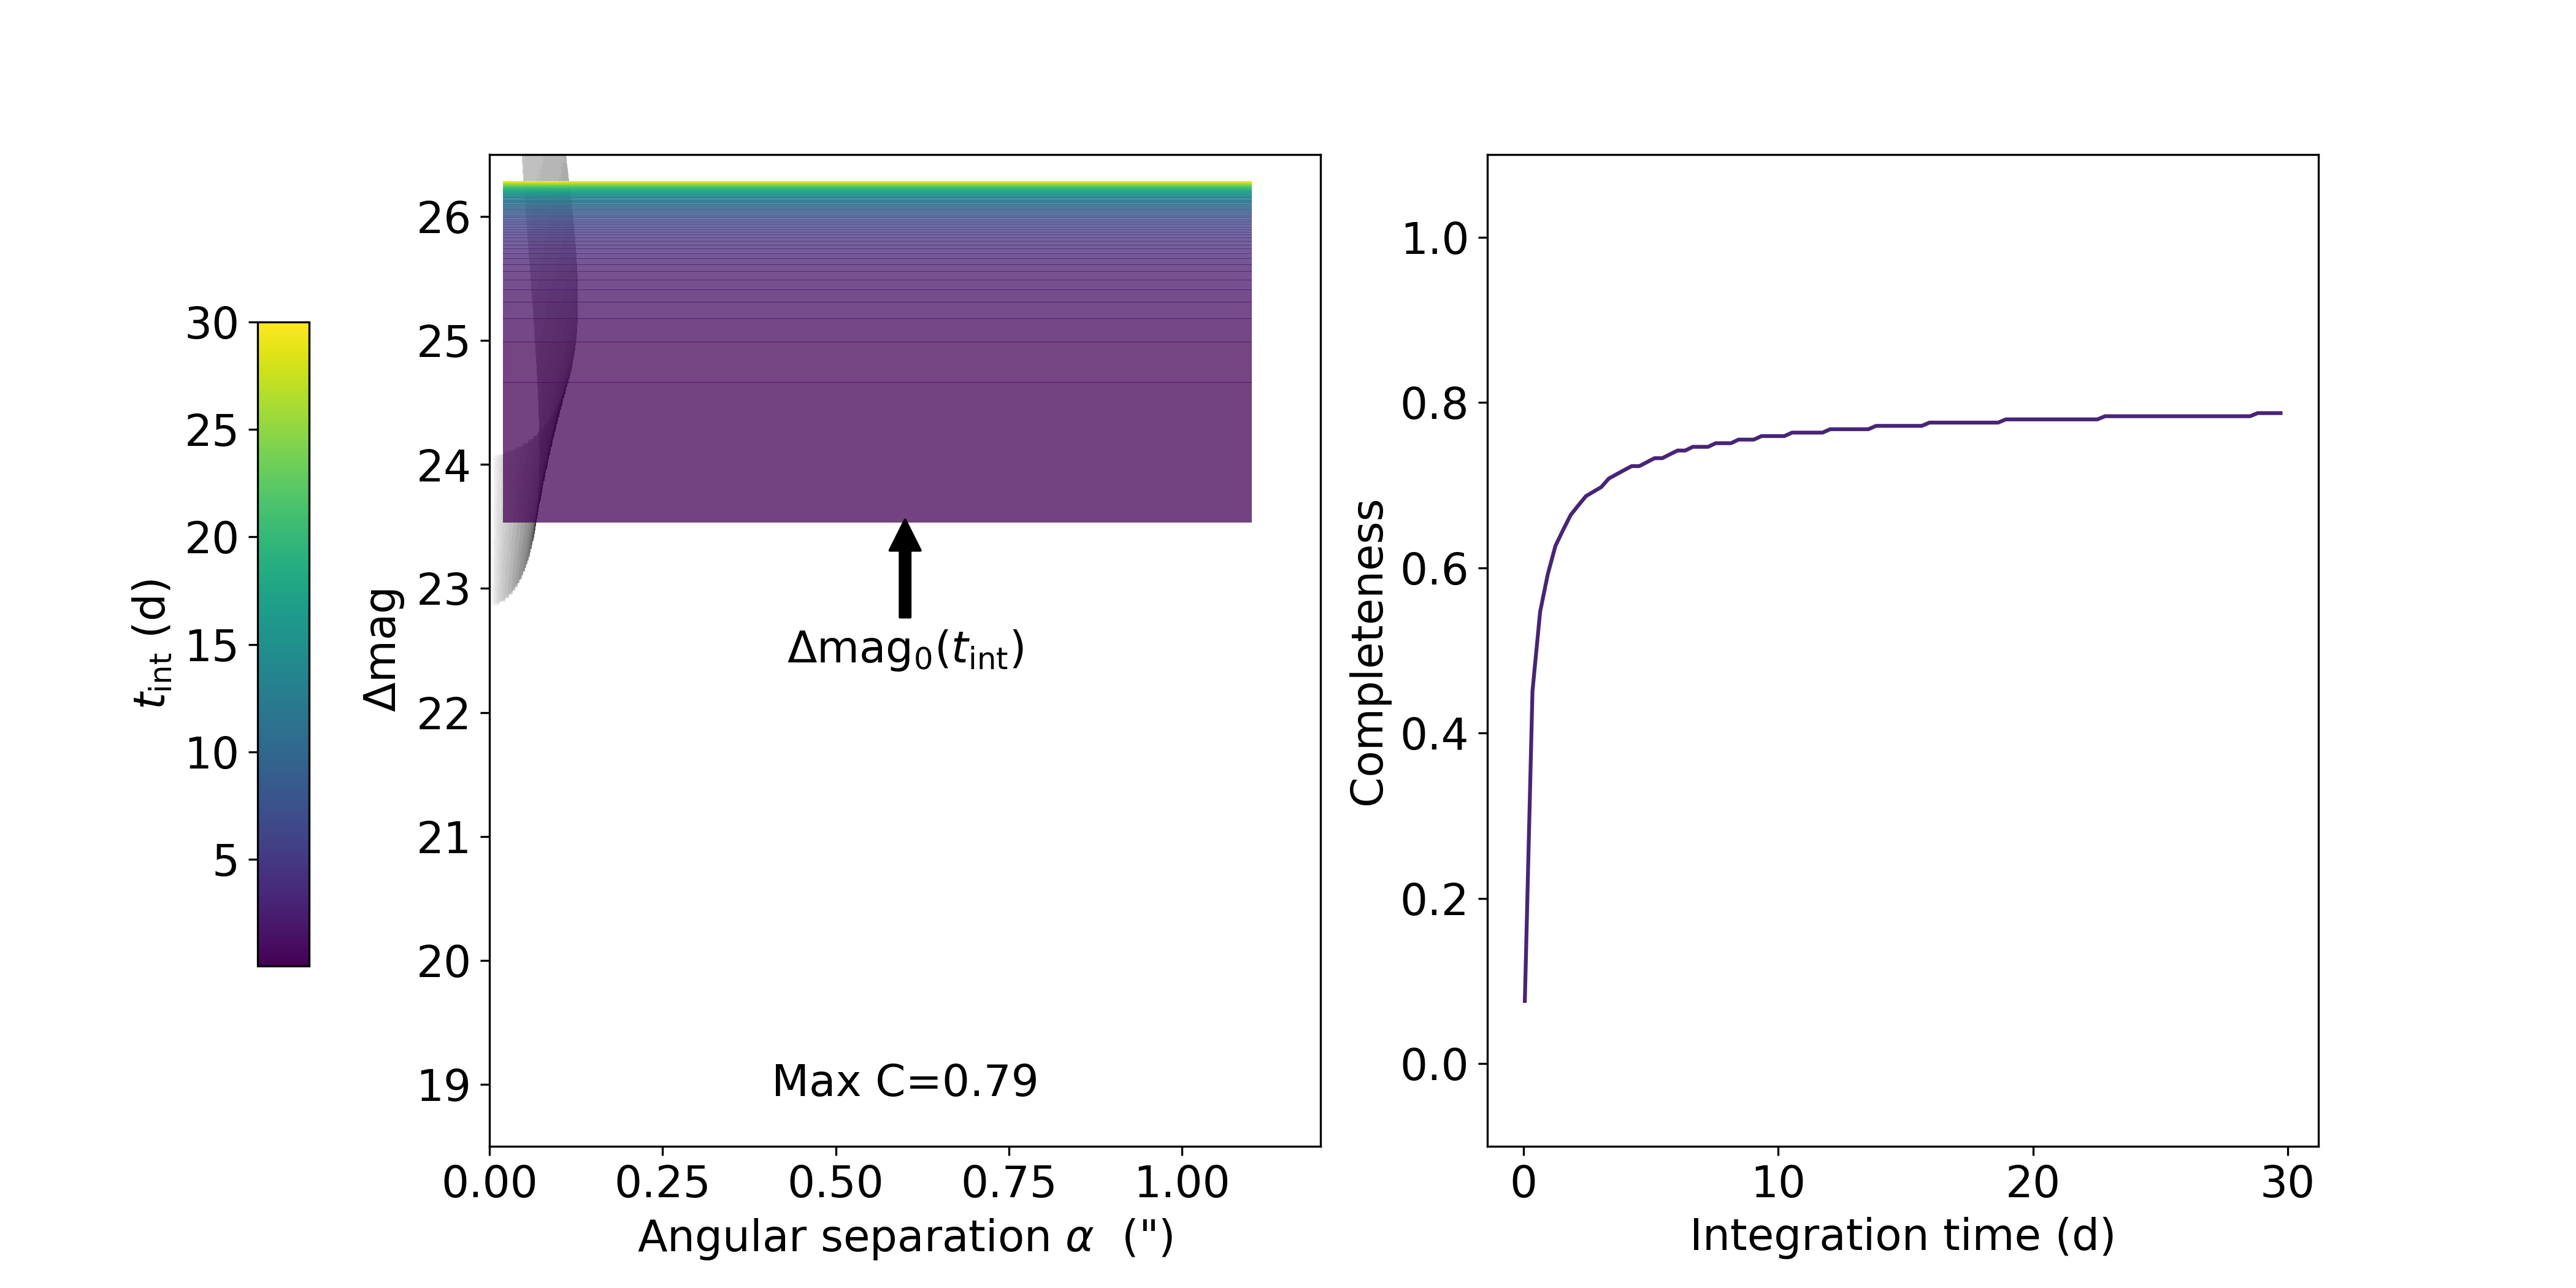
\includegraphics[width=0.95\textwidth]{ch3/figures/default_dmag_curve.png}
  \end{center}
  \caption{Plot of $\Delta\textrm{mag}_0(t_\textrm{int})$ values without separation dependence
  overlaid on the PDF of an Earth-like planet HIP 91438 ($\approx$13 parsecs from Earth)
  if observed with a prospective design of the Habitable Worlds Observatory.
  Completeness for 30 days of integration time is 0.8.}
  \label{fig:default_dmag_curve}
\end{figure}

A good place to start is calculating completeness
as a function of integration time $t_\textrm{int}$. An example
is shown in \Cref{fig:default_dmag_curve}, where the colored rectangle
represents the calculated $\Delta\textrm{mag}_0$ values for a range of
$t_\textrm{int}$ values with $\alpha$ held constant to the mid point between
the IWA and OWA, $n_\textrm{EZ}=22 \frac{\textrm{mag}}{\textrm{arcsec}^2}$, and
$n_\textrm{Z}=23 \frac{\textrm{mag}}{\textrm{arcsec}^2}$. Because we have a
flat $\Delta\textrm{mag}_0$ the completeness can be calculated as
\begin{equation}
  c(t_\textrm{int}) = \int_{0}^{\Delta\textrm{mag}_0(t_\textrm{int})} 
  \int_{\alpha_\textrm{min}}^{\alpha_\textrm{max}} 
  f(\alpha, \Delta\textrm{mag})\textrm{d}\alpha \textrm{d}\Delta\textrm{mag}
  \label{eq:flat_comp_integral}
\end{equation}
where $f(\alpha, \Delta\textrm{mag})$ is the joint probability density function 
of an Earth-like planet population. In this scenario we see a very steep slope
initially and then little benefit after a few days of integration time.

% To reduce computation time
% $\Delta\textrm{mag}$ for a set of logarithmically spaced integration times we
% can interpolate smoothly and get the dimmest detectable $\Delta\textrm{mag}$
% for the star at an required integration time.



\subsection{Zodiacal light calculations}
\label{sub:zodi}

Local and exozodiacal light are calculated in the same manner as is used by
\code{EXOSIMS}, which is based on the work in \citet{leinert1997Reference1998,
starkMaximizingExoEarthCandidate2014,starkLowerLimitsAperture2015,
keithlyOptimalScheduling2020}. The specific intensity of local zodiacal
light is calculated as
\begin{equation}
  I_\textrm{zodi}(\Delta \lambda_\odot, \beta_\odot, \lambda_0) = 
  I_{\textrm{zodi}, \textbf{r}}^V(\Delta \lambda_\odot, \beta_\odot) 
\frac{I_{\textrm{zodi}, \lambda} (\lambda_0)}{I_{\textrm{zodi}, \lambda}(\textrm{500 nm})}
  \label{eq:local_zodi}
\end{equation}
where $I_{\textrm{zodi}, \lambda}$ is an interpolant over
\citet{leinert1997Reference1998} Table 19 for the specific intensity of
zodiacal light as a function of wavelength, $I_{\textrm{zodi},
\textbf{r}}^V(\Delta \lambda_\odot, \beta_\odot)$ is an interpolant over Table 17 of the same
paper and represents the specific intensity of zodiacal light as a function of
the telescope's look vector, $\Delta \lambda_\odot$ is the ecliptic
longitude of the target with respect to the current longitude of the sun,
$\beta_\odot$ is the ecliptic latitude, and $\lambda_0$ is the observing
wavelength. The units for \Cref{eq:local_zodi} are photons/s/m$^2$/as$^2$/nm.
For clarity we will describe the zodiacal light in magnitude units by
converting the specific intensity into mag/as$^2$ units
\begin{equation}
  Z = -2.5 \log_{10}(I_\textrm{zodi}) \,.
  \label{eq:zodi_mag}
\end{equation}

The values of exozodical light are calculated in a
similar fashion but with a multiplication factor $n_{EZ}$ to allow for
planetary systems with more or less dust than the solar system. The calculation
for the specific intensity of exozodiacal light in V band is
\begin{equation}
  I_\textrm{exozodi}^V = n_{EZ} \mathcal{F}_{0,V}10^{-0.4(M_V-M_{V,\odot}+x)}\left( \frac{1 \textrm{AU}}{r}\right)^2
  \label{eq:exozodi}
\end{equation}
where $n_{EZ}$ is the number of zodi in the planetary system (where 1 "zodi" is
equivalent to the exact distribution of dust in the solar system), $M_V$ is the
absolute magnitude of the target star, $M_{V,\odot}$ is the absolute magnitude
of the sun, $x$ is the nominal specific brightness of the planetary system's
disk at 1 AU ($22\textrm{ mag }\textrm{as}^{-2}$), and $r$ is the planet's orbital radius at the time of
observation. To get the specific intensity at an arbitrary wavelength we can
then use $I_\textrm{exozodi}^V$ instead of $I_{\textrm{zodi}, \textbf{r}}^V$ in
\Cref{eq:local_zodi}. To calculate the specific intensity of the planet at a
given time we calculate its $r$ value and the corresponding specific intensity.
In this paper we parameterize the exozodi values with the $n_{EZ}$ value. To
sample $n_{EZ}$ we use the distribution of exozodi from
\citet{ertelHOSTSSurvey2020} which extrapolates the results of the Large
Binocular Telescope Interferometer's (LBTI) "Hunt for Observable Signatures of
Terrestrial planetary Systems" (HOSTS) survey to get a distribution of
exozodical dust.


% Extra zodiacal light is unlikely to be known before a mission, but
% is worth keeping as an input so that different scenarios can be tested quickly.
% The zodiacal light can be estimated as a function of time if a telescope's
% orbit is known. However, in summed completeness simulations the time of
% observation is generally not considered so it would be of little use. 

\subsection{Full Photometric Constraint}
\label{sub:full_comp}
\begin{figure}
  \begin{center}
    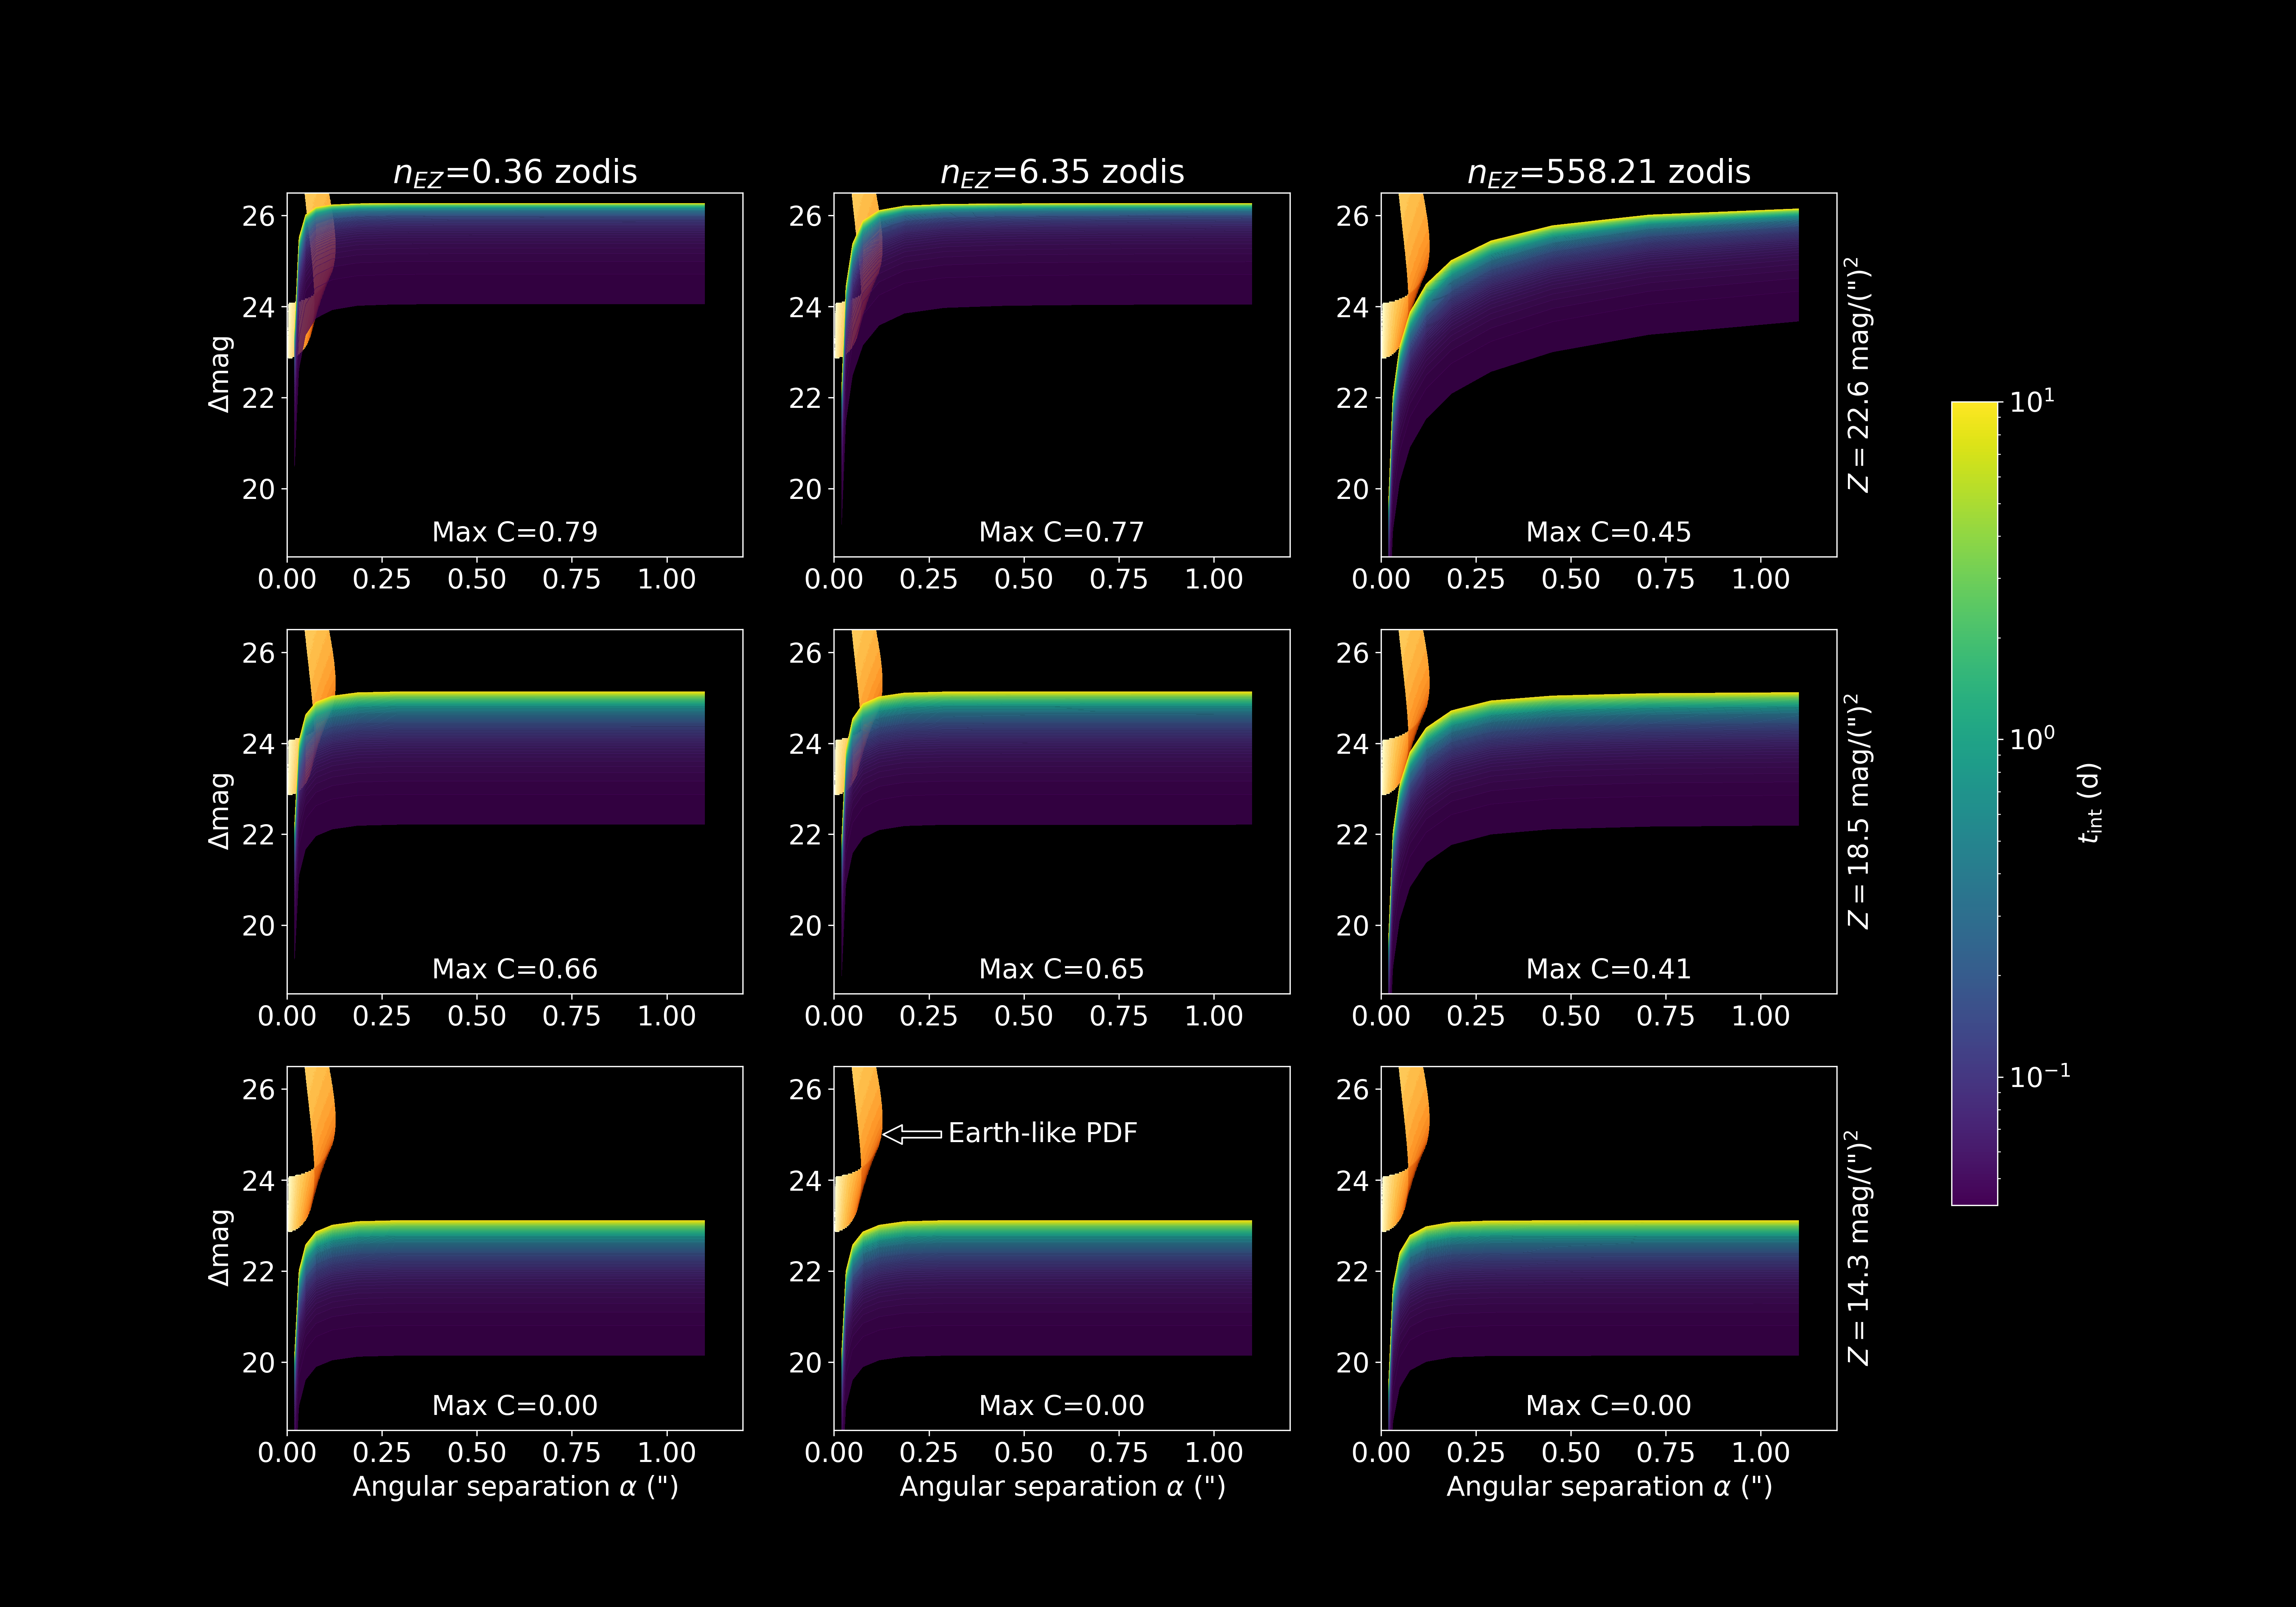
\includegraphics[width=0.95\textwidth]{ch3/figures/fZ_fEZ_curves.pdf}
  \end{center}
  \caption{$\Delta\textrm{mag}_0(t_\textrm{int}, \alpha, Z, n_\textrm{EZ})$ for HIP 91438.
    Each column has a constant value of $n_\textrm{EZ}$ and each row has a
    constant value of $Z$. The zodiacal light values were generated
    using EXOSIMS to simulate the range of zodiacal light values of observing
  the star for a telescope at L2.}
  \label{fig:fZ_fEZ_curves}
\end{figure}

By accounting for integration time, separation, local zodiacal light, and 
exozodiacal light we end up with a four dimensional photometric constraint for
each star, $\Delta\textrm{mag}_0(t_\textrm{int}, \alpha, Z,
n_\textrm{EZ})$. These four dimensions are the range of input values necessary
to invert the exposure time calculator described by \citet{Nemati2014} for a
specific mission design. An example of the $\Delta\textrm{mag}_0$ curves for
various zodiacal light assumptions is shown in \Cref{fig:fZ_fEZ_curves}. 
To visualize the impact of separation and zodiacal light on completeness
we can formulate our limiting $\Delta\textrm{mag}$ as 
$\Delta\textrm{mag}_0(t_\textrm{int}, \alpha, Z, n_\textrm{EZ})$.
Then our equation for completeness becomes
\begin{equation}
  c(t_\textrm{int}, Z, n_\textrm{EZ}) = 
  \int_{\alpha_\textrm{min}}^{\alpha_\textrm{max}} 
  \int_{0}^{\Delta\textrm{mag}_0(t_\textrm{int}, \alpha, Z, n_\textrm{EZ})}
  f(\alpha, \Delta\textrm{mag})\textrm{d}\alpha \textrm{d}\Delta\textrm{mag}
  \label{eq:comp_integral}
\end{equation}
where we leave our zodiacal light values as inputs. In the best case scenario
the completeness is within 0.01 of the flat curve shown in
\Cref{fig:default_dmag_curve}, but drops considerably for high exozodiacal
light values.

\begin{figure}
  \begin{center}
    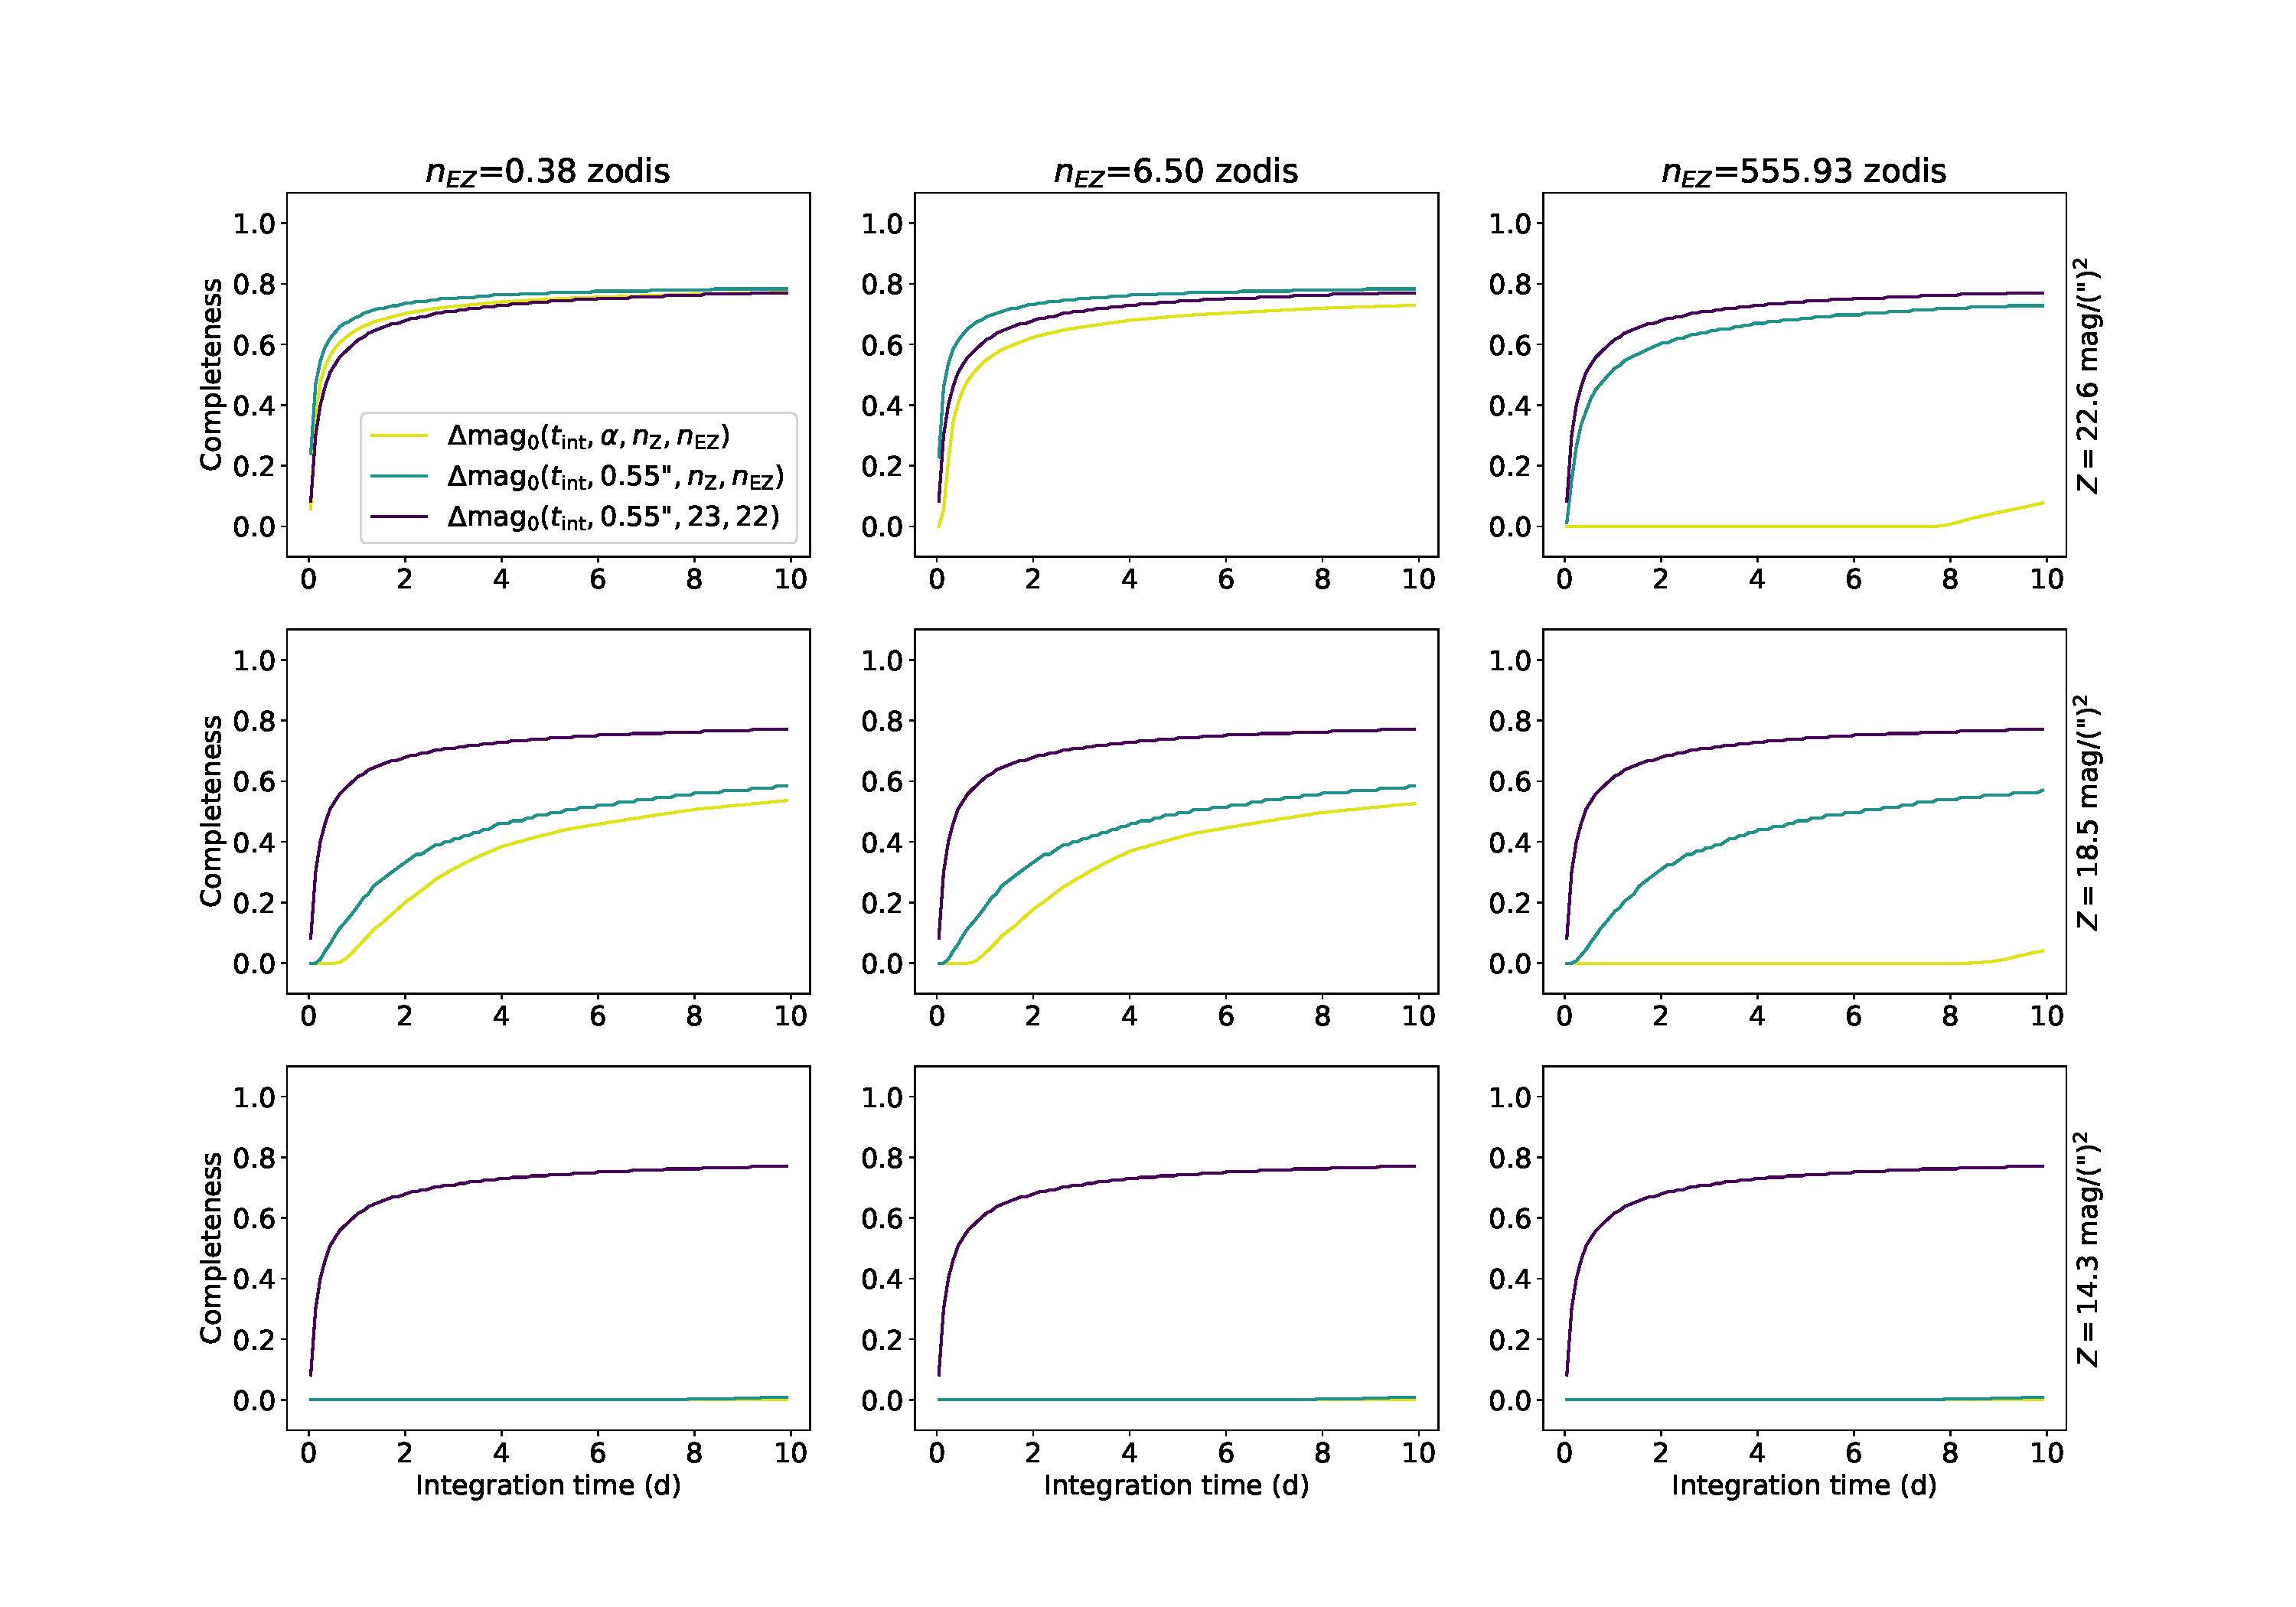
\includegraphics[width=\textwidth]{ch3/figures/Z_EZ_comps_flat.pdf}
  \end{center}
  \caption{Completeness as a function of integration time for the same astrophysical
  scenarios as in \Cref{fig:fZ_fEZ_curves}. The three lines represent different levels
  of accounting for separation and zodiacal light. The line for
  $\Delta\textrm{mag}_0(t_\textrm{int}, \alpha, Z, n_\textrm{EZ})$
  is the most accurate as it accounts for the most variables and is 
  found by applying \Cref{eq:comp_integral} to the curve in \Cref{fig:fZ_fEZ_curves}.
  The 
  $\Delta\textrm{mag}_0(t_\textrm{int}, 0.55", Z, n_\textrm{EZ})$
  line shows the effect of calculating the completeness without accounting for
  the drop in $\Delta\textrm{mag}_0$ at small separations. And the
  $\Delta\mathrm{mag}_0(t_\mathrm{int}, 0.55$"$, 23 (\textrm{mag}/")^2, 22(\textrm{mag}/")^2)$
  line is an overlay of the curve generated in \Cref{fig:default_dmag_curve}.
  }
  \label{fig:fZ_fEZ_comps}
\end{figure}

\begin{figure}
  \begin{center}
    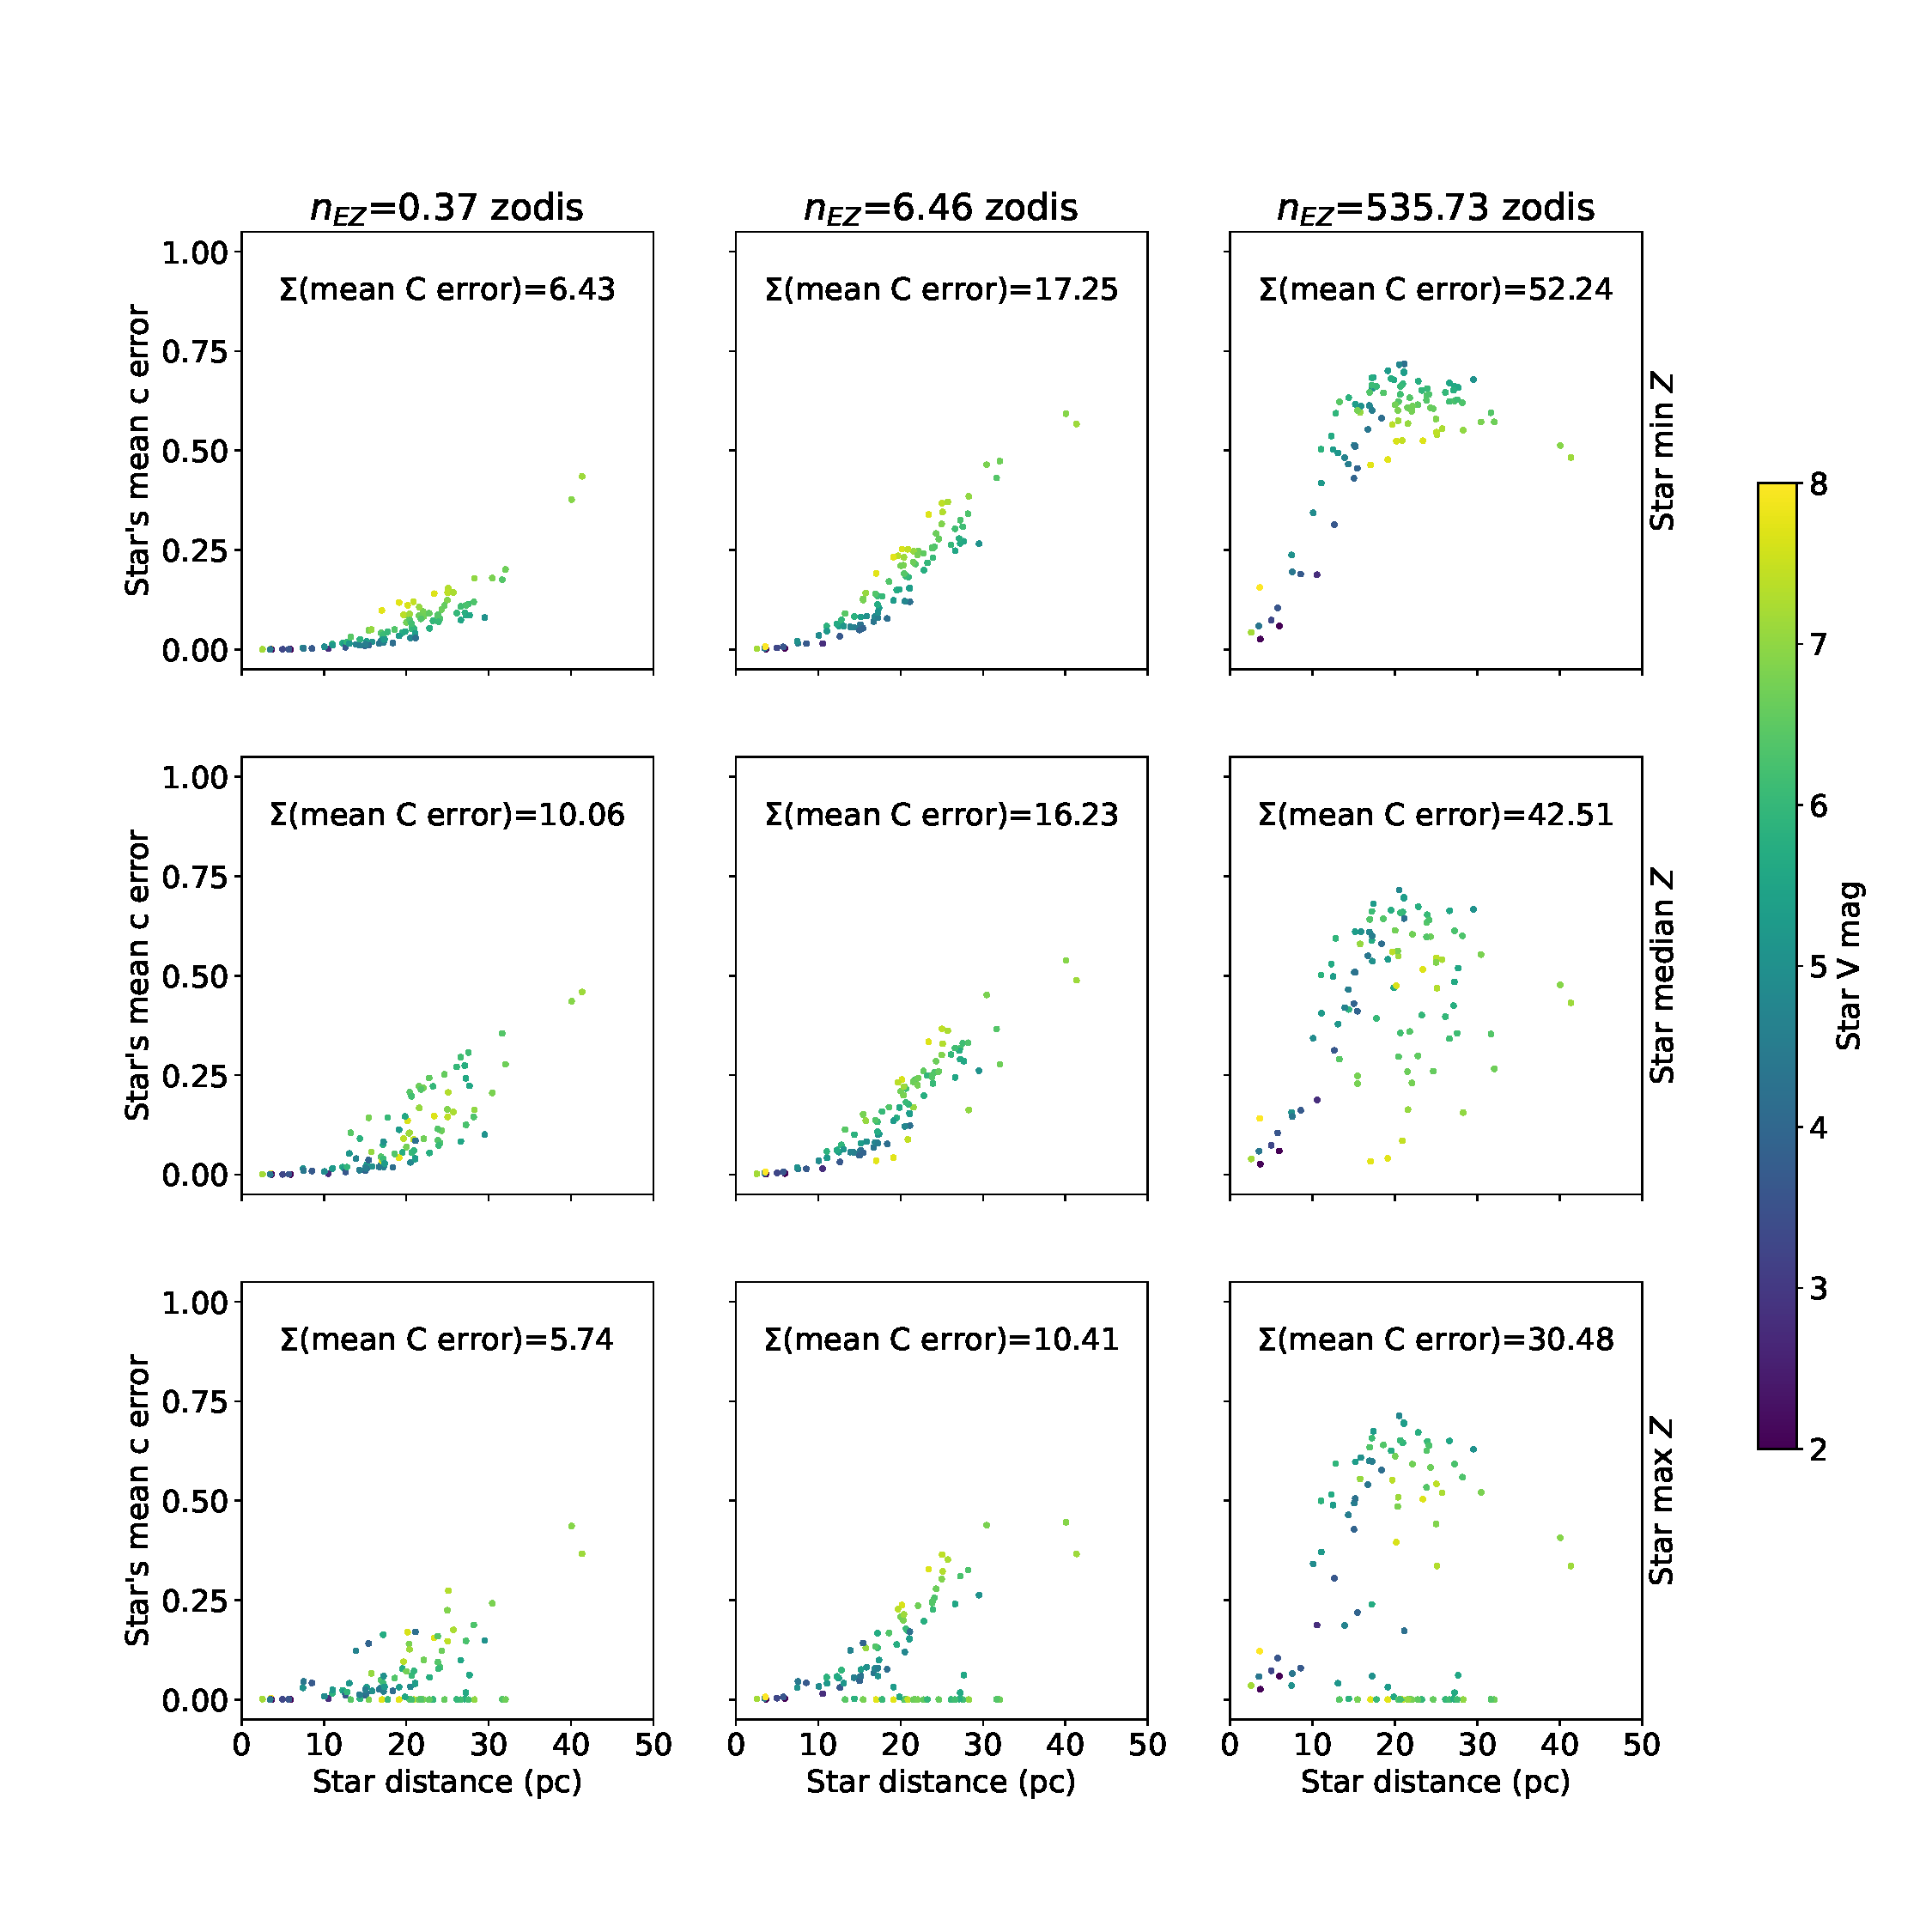
\includegraphics[width=0.95\textwidth]{ch3/figures/mean_comp_errors.pdf}
  \end{center}
  \caption{Mean completeness error for different stars calculated as the mean difference between
  the default curve and the scenario curve in \Cref{fig:fZ_fEZ_comps} for each star. The columns represent
  different amounts of exozodiacal dust and the rows show the star's minimum, median, and maximum zodiacal
  light surface brightness for a telescope on an L2 orbit. The increase in 
  mean completeness error as star distance increases shows that not accounting for the effects of
  $\alpha$ on $\Delta\textrm{mag}_0$ leads to a systematic overestimation of completeness. 
  The effect becomes more pronounced for greater amounts of exozodiacal dust 
  assumed.}
  \label{fig:mean_comp_errors}
\end{figure}

To see the effect on completeness more clearly \Cref{fig:fZ_fEZ_comps} shows
completeness as a function of integration time for the various scenarios in
\Cref{fig:fZ_fEZ_curves} and compares them to the completeness curves generated
with less complete information. All of the values shown in
\Cref{fig:default_dmag_curve,fig:fZ_fEZ_curves,fig:fZ_fEZ_comps} are for a
single star and demonstrate the large trade space inherent to making
assumptions on the zodiacal light when maximizing completeness. Without
ensuring that observations are made near the minimum local zodiacal light value
a high completeness observation can drop to zero completeness. Values of
exozodiacal light are unlikely to be known before an initial observation is
made so it cannot be accounted other than choosing an assumed $n_\textrm{EZ}$
value.

\Cref{fig:mean_comp_errors} summarizes the effect of using the optimistic
"default" scenario of a flat limiting $\Delta\textrm{mag}$ per integration time. The targets shown are the 97 stars from the NEID Earth Twin Survey with
full stellar information in the Simbad database
\citep{guptaTargetPrioritization2021}. For each star the $\Delta\textrm{mag}_0$
values are generated. Then the completeness per integration time function is
generated for both the case when $\Delta\textrm{mag}_0$ is assumed to be flat
and the case that takes separation into account, similar to
\Cref{fig:fZ_fEZ_comps}. We average the distance between the two completeness
per integration time functions and plot them as a single point in
\Cref{fig:mean_comp_errors}. It's clear that the change in limiting
$\Delta\textrm{mag}$ near the IWA becomes a problem past 10 parsecs. For
extreme exozodiacal light values the effect becomes much more pronounced.

For yield modeling based on Monte Carlo mission simulations, such as EXOSIMS
\citep{savranskyWFIRSTAFTACoronagraphScience2015, delacroixScienceYield2016,
savranskyEXOSIMSExoplanetOpenSource2017}, the $\Delta\textrm{mag}_0$ values for
a star can be reused across mission simulations with the same telescope orbit
and optical system. Calculating the 2000 $\Delta\textrm{mag}_0$ values to
account for all combinations of 10 $\alpha$ values, 20 $t_\textrm{int}$ values,
and 10 $Z$ values takes 20-30 seconds to run on a Ryzen 5800x 8 core processor
in parallel. An application of this could be to schedule observations when
accounting for the zodiacal light without requiring observations be made at the
zodiacal light minimum, as was done in \citet{keithlyOptimalScheduling2020}. In
that scheduler observations are all made at the minimum zodiacal light for the
target star. By allowing for observations at times near the minimum, the
scheduler can likely make worthwhile trades between targets.

% \subsection{TODO:Exozodi calculations}
% Given a distribution of zodi values for a planetary system we could marginalize
% over it to calculate the completeness with respect to the possible zodi values
% of an unknown planetary system.
% \begin{equation}
%   c(t_\textrm{int}, n_\textrm{Z}) = 
%   \int_{n_\textrm{EZ,min}}^{n\textrm{EZ,max}} 
%   \int_{\alpha_\textrm{min}}^{\alpha_\textrm{max}} 
%   \int_{0}^{\Delta\textrm{mag}_0(t_\textrm{int}, \alpha, n_\textrm{Z}, n_\textrm{EZ})}
%   f(\alpha, \Delta\textrm{mag}) g(n_\textrm{EZ})
%   \textrm{d}\alpha \textrm{d}\Delta\textrm{mag} \textrm{d}n_\textrm{EZ}
%   \label{eq:comp_integral_nEZ}
% \end{equation}
% where $g(n_\textrm{EZ})$ is the density function of $n_\textrm{EZ}$.

% The reason to include separation in the formulation of the photometric
% constraint is shown in The traditional set of dimmest detectable
% $\Delta\textrm{mag}$ values is shown in 

\section{Probability of Detection} % (fold)
\label{section:impact_on_pdet}

An interesting challenge for direct imaging is using the orbit fits from
indirect exoplanet detection techniques to estimate the best times to make
direct observations. Indirect detection via the radial velocity method cannot
separate the mass and inclination of a planet's orbit, which complicates direct
imaging scheduling because the inclination is important for the planet-star
separation and the mass is used to estimate radius which impacts the brightness
of the planet. Chapter 2 showed how to take a radial velocity fit and generate
the most likely times the planet will be detectable for a given instrument.
Notably missing from that work was considerations of integration time and
zodiacal light conditions.

For a star with a planet fitted via the radial velocity method we can calculate
the dimmest detectable $\Delta\textrm{mag}$ curves, the $\Delta\textrm{mag}_0$
values, for a telescope's orbit and optical system by looping over the zodiacal
light values for the star during the mission, the separations between the
instrument's IWA and OWA, and integration times spaced logarithmically between
the minimum and maximum allowed integration times. Logarithmic spacing is
useful as the largest changes in $\Delta\textrm{mag}_0$ occur at small
integration times and because $\Delta\textrm{mag}$ is a logarithmic quantity
while time is linear. In testing we found that the most useful process was
calculating 2d interpolants that return the dimmest detectable
$\Delta\textrm{mag}$ given an integration time and separation. We generate a 2d
interpolant for a set of 10 zodiacal values between the star's minimum and
maximum zodiacal light surface brightness during the telescope's orbit. 

Exozodiacal light is treated similarly to the local zodiacal light in that it
is not included in the interpolants. Unlike the zodiacal light we cannot come
up with the surface brightnesses directly, instead we generate a range of
$n_\textrm{EZ}$ "zodis" as defined by
\citet{starkMaximizingExoEarthCandidate2014} and calculate the 2d interpolants
for a single value of $n_\textrm{EZ}$. For every $\alpha$ in the interpolant
the exozodiacal light surface brightness is calculated as if the planet is at
$\alpha$ value with an inclination of $135\degree$. Calculating it in this
fashion includes the fact that the exozodiacal light decreases for distant
orbits.

Using the dimmest detectable $\Delta\textrm{mag}$ curves to calculate
the probability of detection is useful because it means we do not need to calculate
the signal to noise ratio of every one of the orbit fits at every possible
observation time for all integration times. Instead we propagate to time $t$ in
($\alpha$, $\Delta\textrm{mag}$) space with the method shown in
\Cref{cha:first_paper}, get the interpolant corresponding to the local zodiacal
light for the target star at $t$, and call that 2d interpolant with all the
$\alpha$ and integration times which returns the dimmest detectable
$\Delta\textrm{mag}$ values of interest. Then the probability of detection for
an integration time is a simple percentage of the number of
$\Delta\textrm{mag}$ values from propagation that are above their corresponding
the $\Delta\textrm{mag}_0$ values, or
\begin{equation}
  P_\textrm{det}(t, t_\textrm{int}, Z, n_\textrm{EZ}) = 
  \int_{\alpha_\textrm{min}}^{\alpha_\textrm{max}} 
  \int_{0}^{\Delta\textrm{mag}_0(t_\textrm{int}, \alpha, Z, n_\textrm{EZ})}
  f(\alpha, \Delta\textrm{mag})\textrm{d}\alpha \textrm{d}\Delta\textrm{mag}
  \label{eq:comp_integral}
\end{equation}

\subsection{Validation}

\begin{figure}
  \begin{center}
    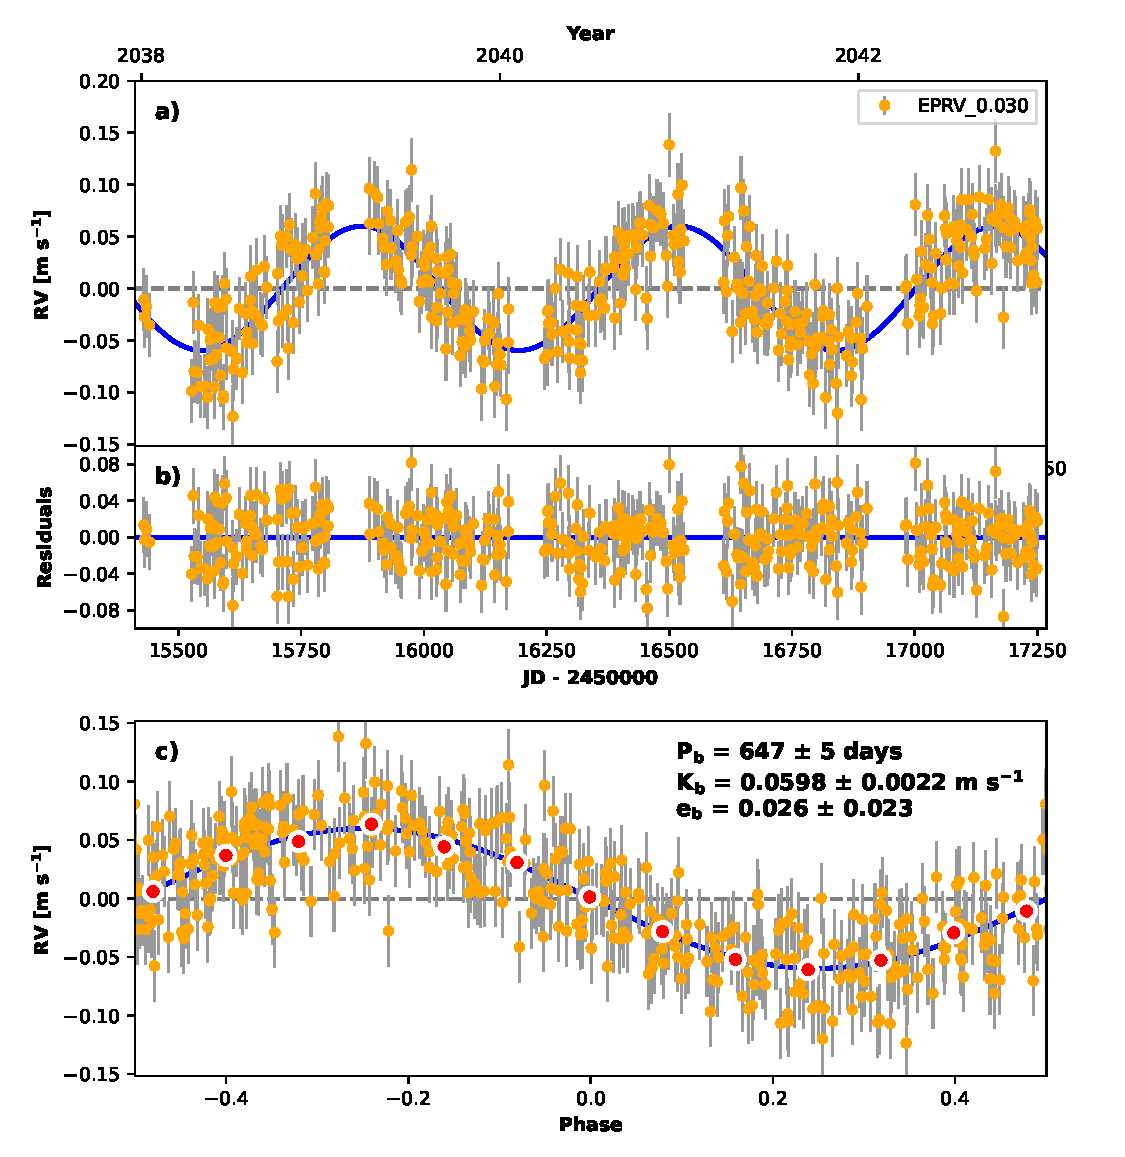
\includegraphics[width=0.95\textwidth]{ch3/figures/orbit_plot_mc_HIP_91438.pdf}
  \end{center}
  \caption{Radial velocity orbit fit of a habitable zone planet on a nearly edge on orbit from
  simulated extreme precision radial velocity data. Fit was done using
  \code{RVSearch}
  \citep{rosenthalCaliforniaLegacy2021}. Top row
  (a) overlays the observed RV data on the fitted planet's RV signal. Middle
  row (b) shows the residual RV signal when the fitted planet's RV signal is
  subtracted. The bottom row (c) shows the fitted planet's signal over a single
  period and the observed RV data's match to the planet signal. The bottom row
  additionally marks the planet's fitted period $P$, eccentricity $e$, and RV
  semi-amplitude $K$. The fit shows strong agreement with the underlying signal
  because the fitted orbital parameters are all within two standard deviations of the true
  planet orbital parameters.}
  \label{fig:rv_fit}
\end{figure}

\begin{figure}
  \begin{center}
    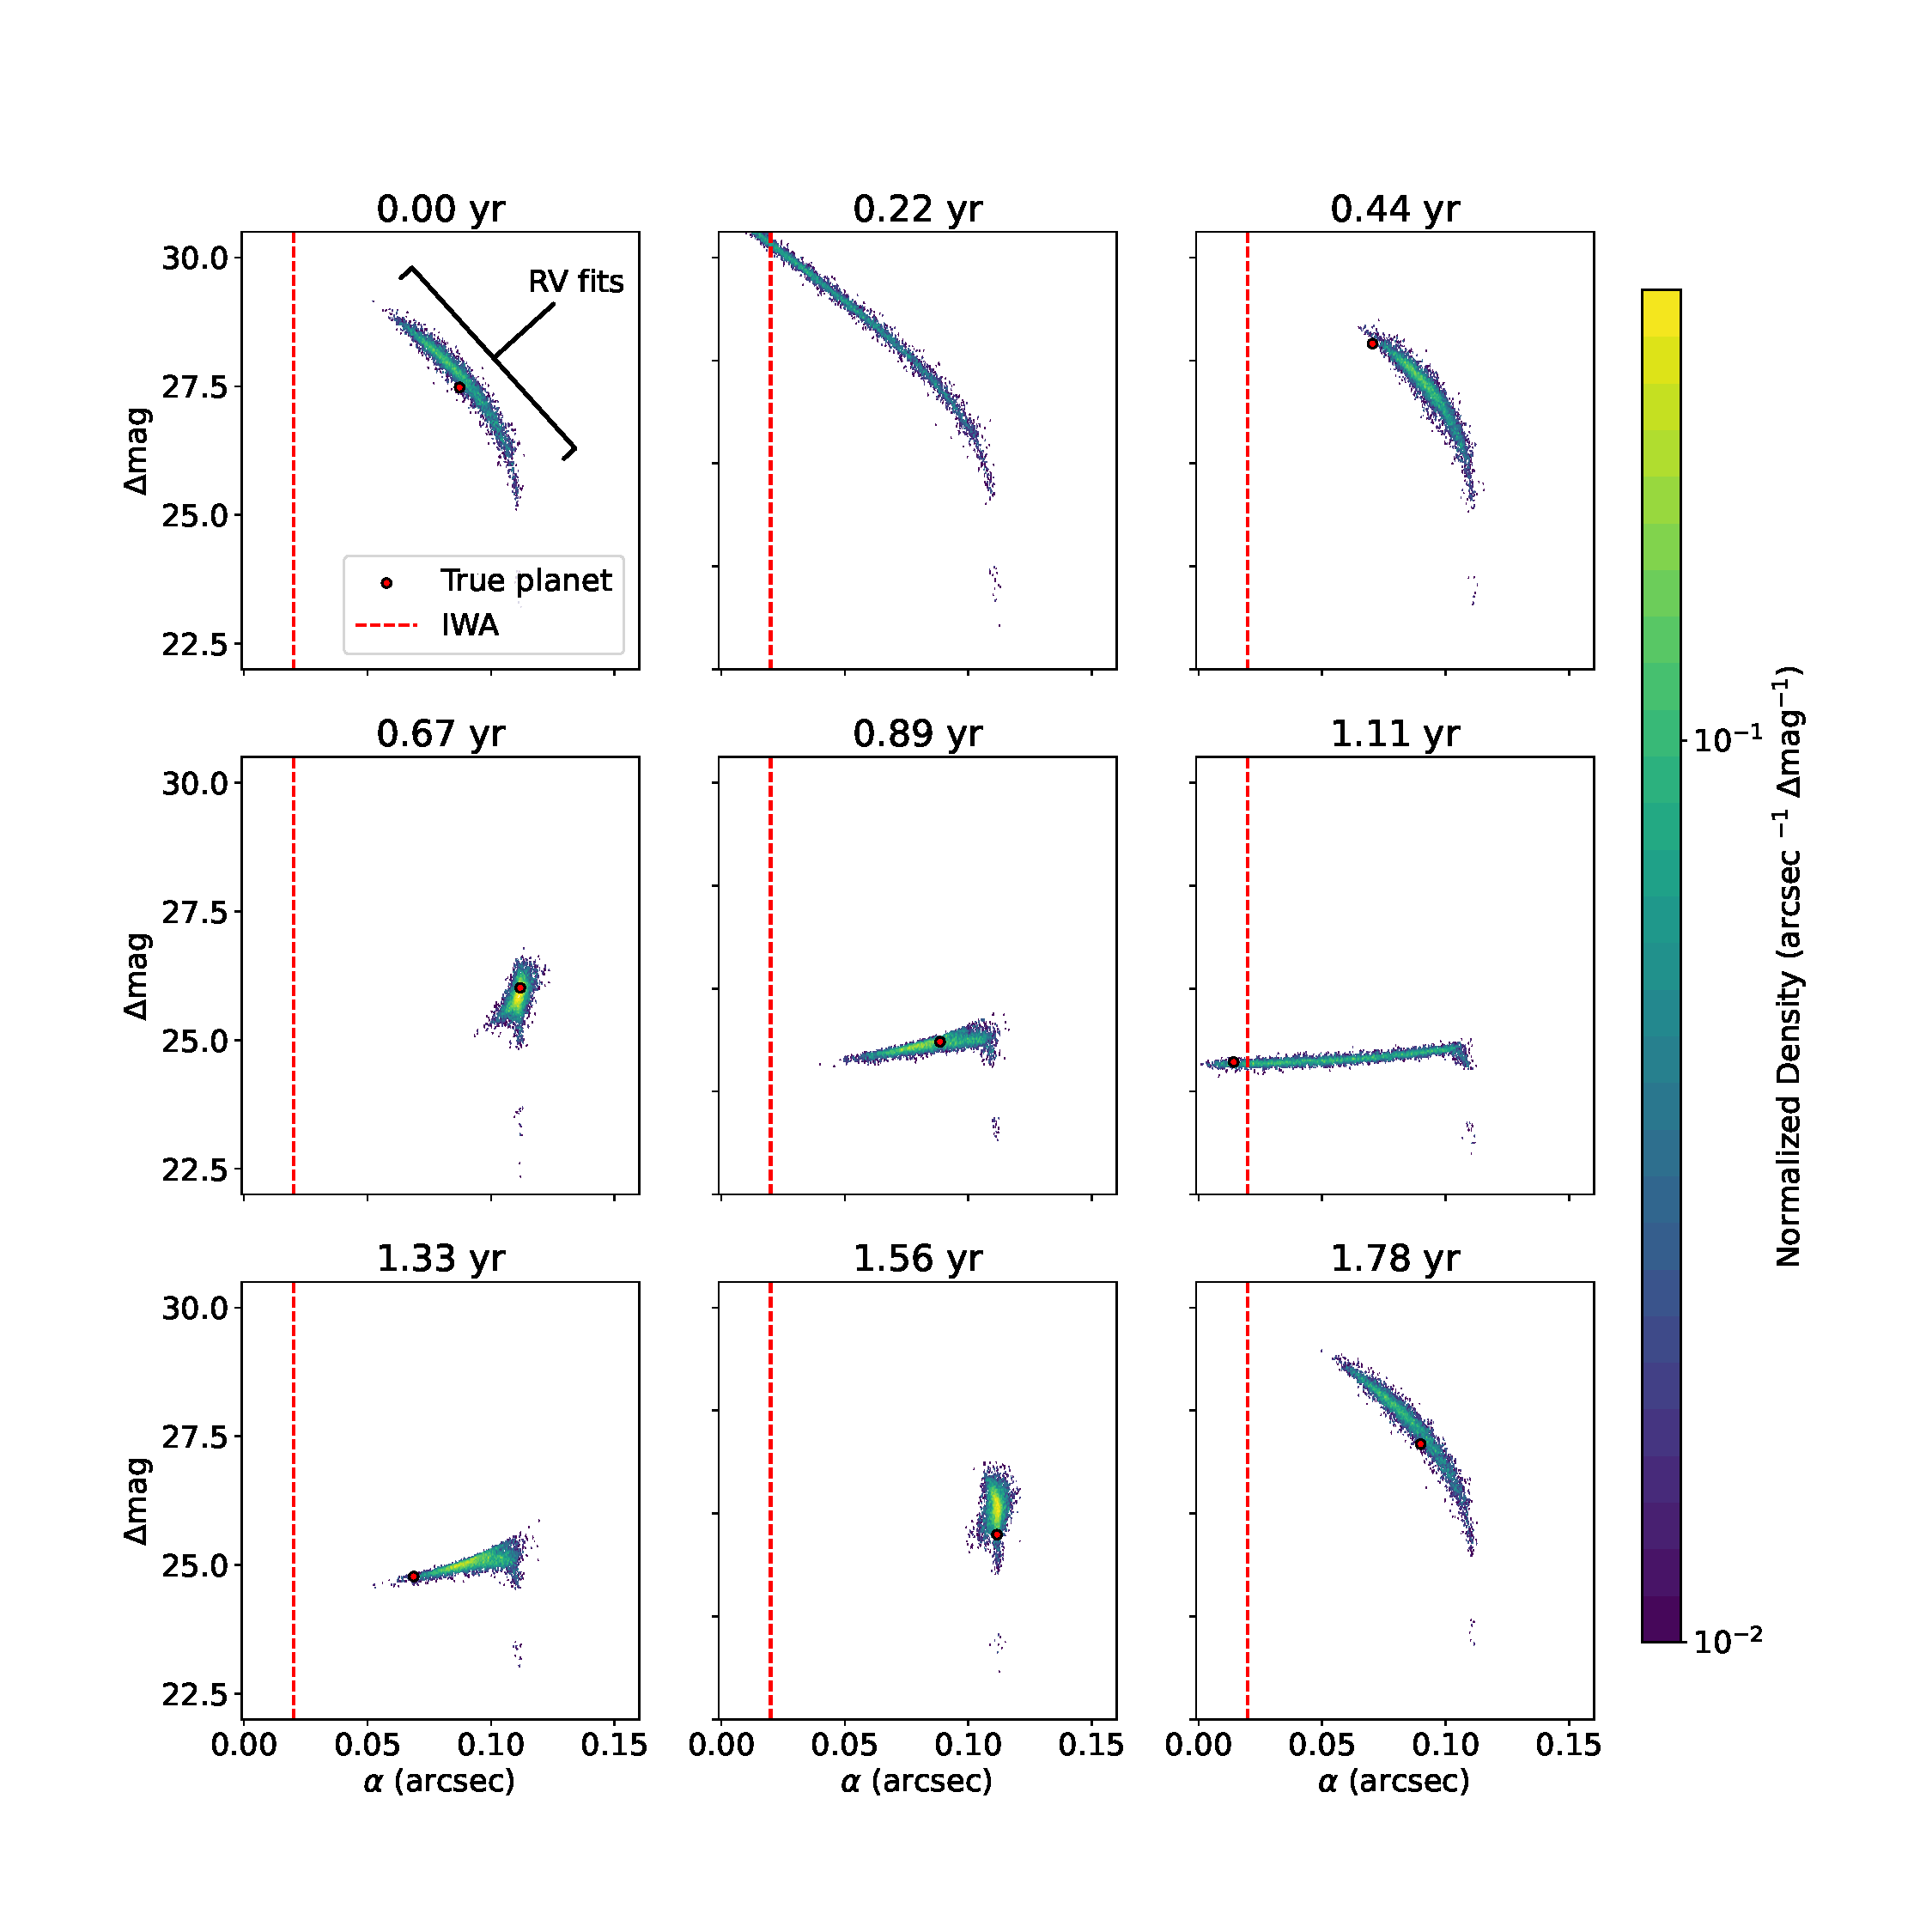
\includegraphics[width=0.95\textwidth]{ch3/figures/pop_propagation_in_time.pdf}
  \end{center}
  \caption{Propagation of the fitted orbits from \Cref{fig:rv_fit} compared to
    the propagation of the true planet. Each subplot is titled with the length
    of time passed since the final RV observation was made. The true planet remains
    within the set of fitted orbits which shows the fitted orbits are
  accurately describing the planet's $\alpha$ and $\Delta\textrm{mag}$ values. Because
  the fit had small errors on the orbital parameters there is very little dispersion
  among the fitted orbits.}
  \label{fig:pop_propagation_in_time}
\end{figure}

\begin{figure}
  \begin{center}
    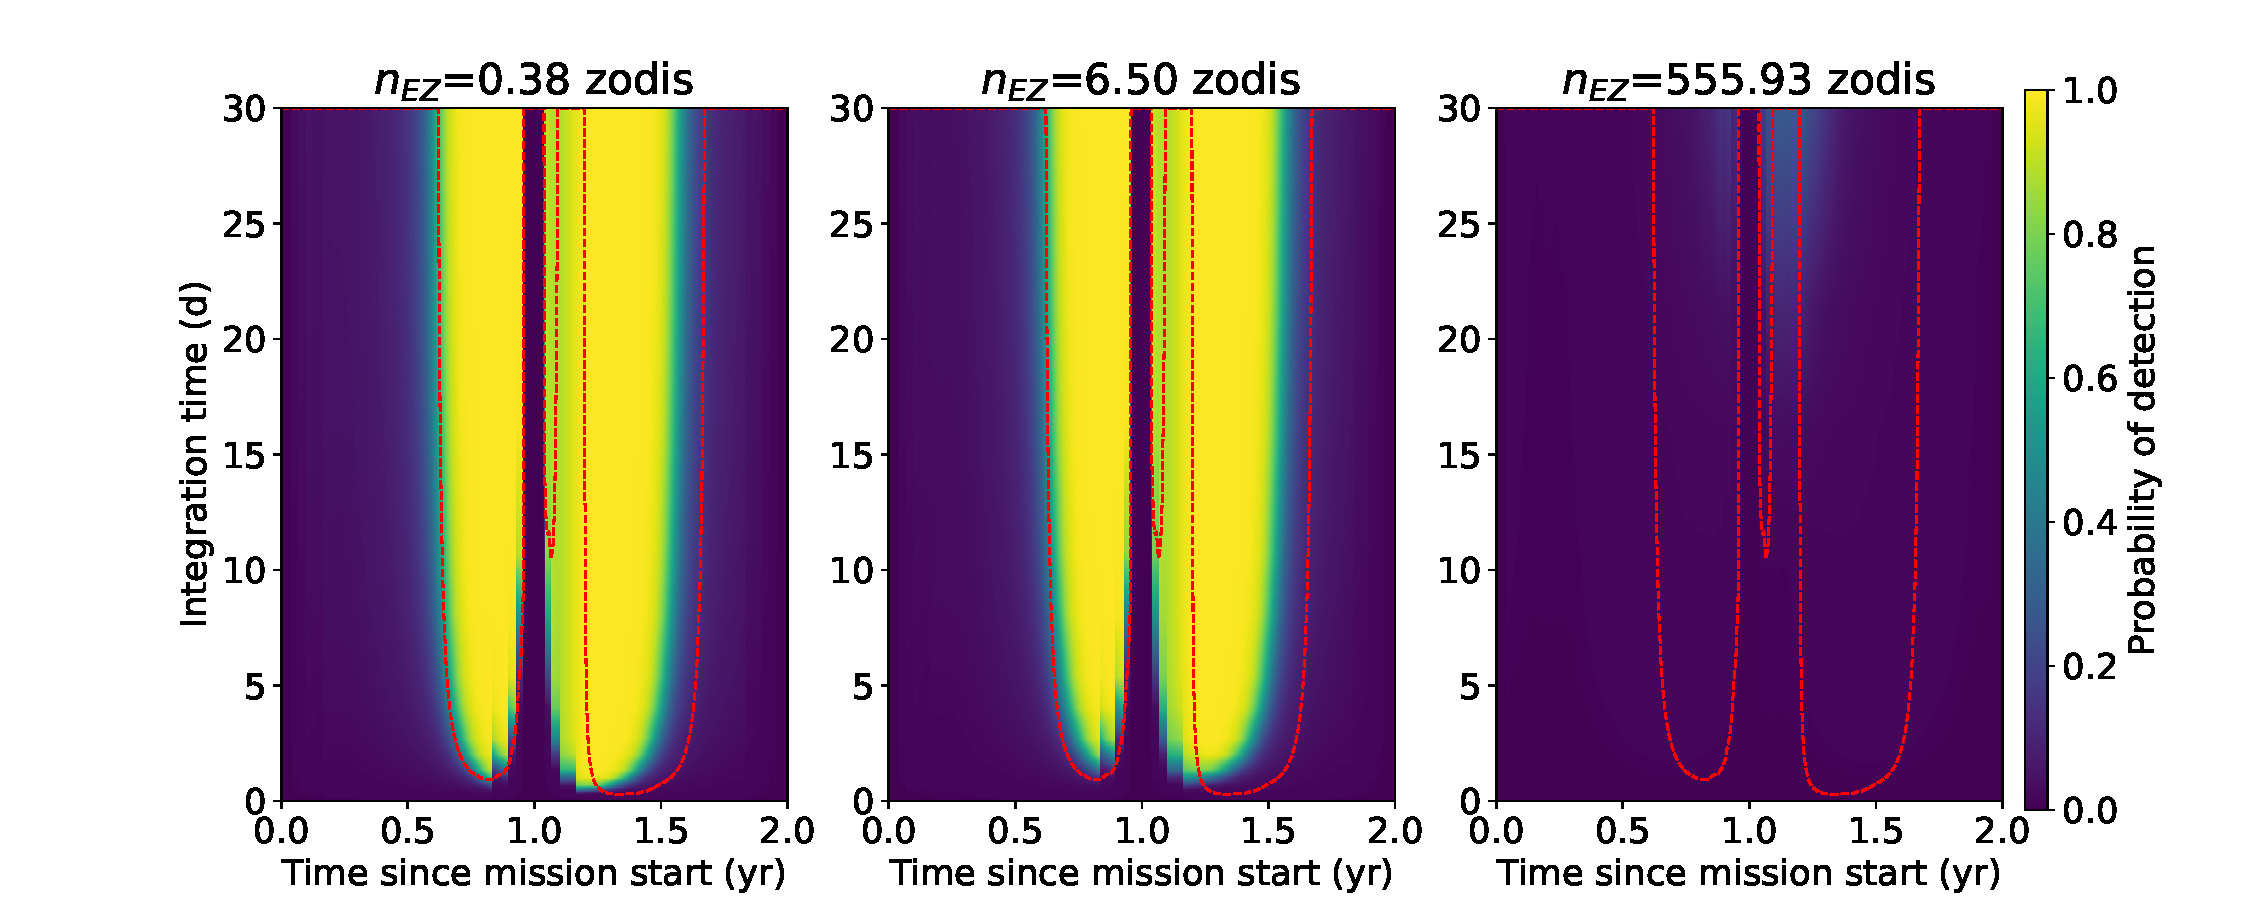
\includegraphics[width=0.95\textwidth]{ch3/figures/pdet_colored_true_overlay.pdf}
  \end{center}
  \caption{Probability of detection values for a 6m telescope similar to the
  projected Habitable Worlds Observatory from \citet{morganExplorationExpectedNumber2022a}
  with the radial velocity fit shown in \Cref{fig:rv_fit}. The
red dotted line represents the true detectability of the planet. Any
observation made outside of the red lines would result in a missed detection.}
  \label{fig:pdet_colored_true_overlay}
\end{figure}

\begin{figure}
  \begin{center}
    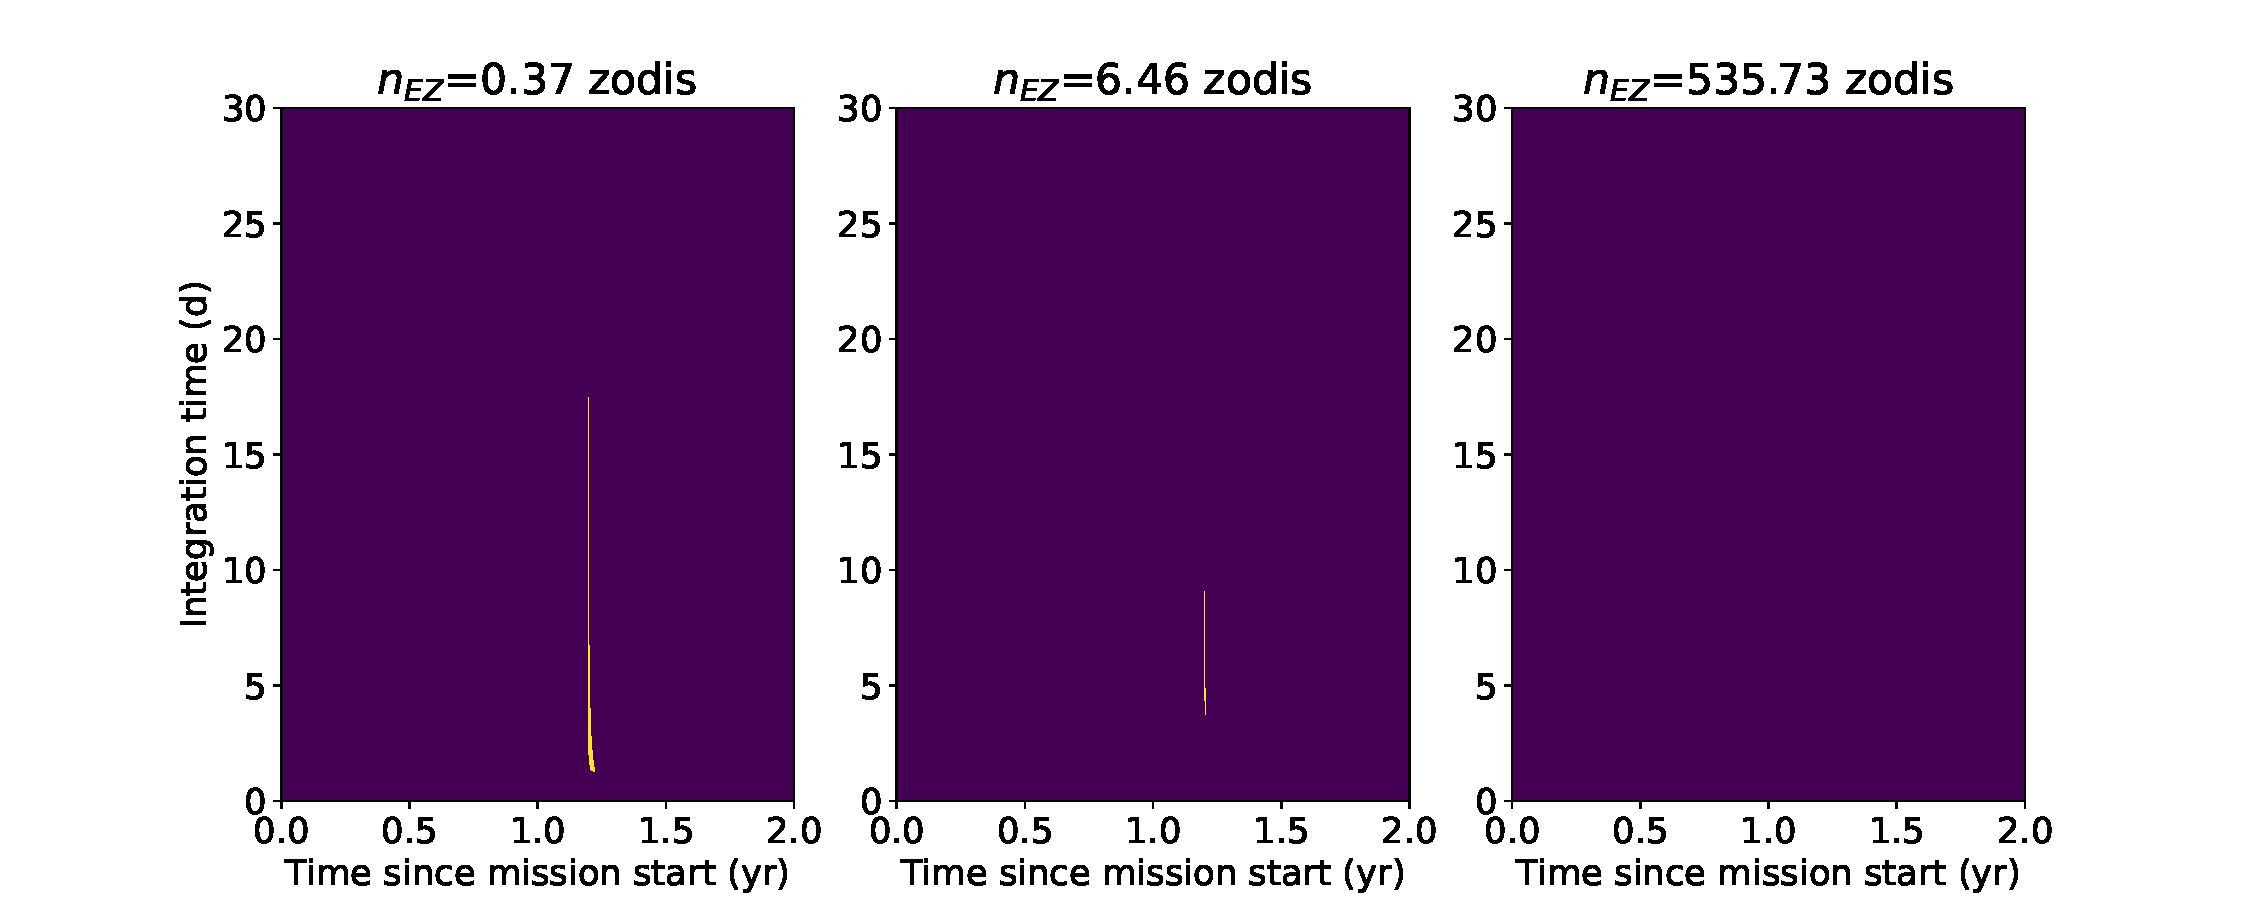
\includegraphics[width=0.95\textwidth]{ch3/figures/pdet_colored_true_err.pdf}
  \end{center}
  \caption{Plot highlighting where the estimated probability of detection is greater
  than 0.99 and the true planet is not detectable. Because very little of the space
  is highlighted this plot shows that the estimated probability of detection is a
  strong predictor of when the true planet is detectable. The only points highlighted
  correspond to when the true planet is exiting the IWA of the coronagraph which a
  scheduling algorithm could account for.}
  \label{fig:pdet_colored_true_err}
\end{figure}


To demonstrate the process we generated synthetic radial velocity data for a
randomly generated planet drawn from occurrence rates from
\citet{dulzJointRadialVelocity2020} fixed to be on a circular orbit. The true
planet parameters are $T=653$ days, $i=91.28\degree$, $M_p=0.79 M_\oplus$, $R_p
= 0.944 R_\oplus$. The RV data was created with precision $\sigma=0.03$ m/s.
The fitting was done with \code{RadVel} \citep{fultonRadvelRadialVelocity2018}
via the \code{RVSearch} package \citep{rosenthalCaliforniaLegacy2021} as shown in \Cref{fig:rv_fit}. A set of 10,000 orbits consistent with the RV
fit were created using the "credible interval" method from Chapter 2 and
propagated in time as shown in \Cref{fig:pop_propagation_in_time}.

The process of using the full photometric constraint from \Cref{sub:full_comp} for
$P_\textrm{det}$ gives us the probability of detecting the
fitted planet as a function of both observation and integration time, shown in
\Cref{fig:pdet_colored_true_overlay}. The plot includes the detectability of
the true planet, calculated using EXOSIMS, which shows strong agreement with
the calculated probability of detection based on the RV fit. The only major
section where the probability of detection is high and the planet is not
detectable is when the true planet is inside the inner working angle around 1.1
years. This is shown in \Cref{fig:pop_propagation_in_time} and while the
estimated probability of detection is high it is not unity, because the
sampling of orbital inclination described in Chapter 2 captures the fact that
only very edge-on orbits will be inside the inner working angle. We show
the areas where the calculated probability of detection is above 0.99 and the
true planet is not detectable in \Cref{fig:pdet_colored_true_err}, which
shows that the model does a very good job of capturing the true detectability
of the planet with only a small range of values where the model and the true
detectability do not line up while the planet is near the telescope's IWA.

\Cref{fig:pdet_colored_true_err} further shows how the assumption on
exozodiacal light impacts the resulting probability of detection, functioning
similar to a safety factor. Choosing a high $n_\textrm{EZ}$ value results in
depressed probability of detection values in exchange for more guarantee that
any individual observation will be successful.

% section section:Observing scenario specific probability of detection (end)

\section{Conclusion} % (fold)
\label{sec:con_ddMag_comp}

In this chapter we motivated the need to account for more astrophysical
parameters to estimate the probability of directly imaging a planet detected
with RV. We started by making an analogy to the completeness metric, a single
value to represent the likelihood of a detecting a planet from an assumed
population given a specific star and mission design, to show that separation
and zodiacal light values have a considerable impact. If those effects are not
accounted for a yield study using summed completeness will systematically
overestimate the number of planets the mission will find. Then by calculating
$\Delta\textrm{mag}_0$ as a function of integration time, angular separation,
zodiacal light, and exozodiacal light we showed that we can very accurately
estimate the observation and integration times necessary to directly image an
exoplanet. For a direct imaging mission scheduler this level of detail in the
probability of detecting a planet is very important because it shows the trade
space between the observing time and integration time available for a specific
target. Making an optimal schedule requires efficient use of observation time
and this process of calculating the probability of detection can be used to
increase the number of planets a direct imaging mission detects.

% section ch3_discussion (end)
